% This is based on the LLNCS.DEM the demonstration file of
% the LaTeX macro package from Springer-Verlag
% for Lecture Notes in Computer Science,
% version 2.4 for LaTeX2e as of 16. April 2010
%
% See http://www.springer.com/computer/lncs/lncs+authors?SGWID=0-40209-0-0-0
% for the full guidelines.
%
\documentclass[a4paper,11pt]{article}
\usepackage[osf]{mathpazo}
\usepackage{ms}
\usepackage[numbers, sort&compress]{natbib}
\usepackage{lineno}
\usepackage{graphicx}
\usepackage{upgreek}
\usepackage{caption}
\usepackage[osf]{mathpazo}
\usepackage[T1]{fontenc}
\usepackage{textcomp}
\modulolinenumbers[5]
\linenumbers

\pdfminorversion=3

\makeatletter
\renewcommand{\@biblabel}[1]{\quad#1.}
\makeatother

\newcommand{\E}{\mathrm{E}}
\newcommand{\Var}{\mathrm{Var}}
\newcommand{\Cov}{\mathrm{Cov}}
\newcommand{\kronecker}{\raisebox{1pt}{\ensuremath{\:\otimes\:}}} 

\title{The evolution of energetic scaling across the vertebrate tree of life}
\author{Josef C. Uyeda$^{1,*}$, Matthew W. Pennell$^{1,2}$, Eliot T. Miller$^{1,3}$, \\Rafael Maia$^{1,4}$, \& Craig R. McClain$^5$}

\date{}
\affiliation{
$^{1}$ Department of Biological Sciences \& Institute for Bioinformatics and Evolutionary Studies, University of Idaho, Moscow, ID 83844, U.S.A. \\
$^{2}$ Department of Zoology and Biodiversity Research Centre, University of British Columbia, Vancouver, BC V6T 1Z4, Canada\\
$^{3}$ Cornell\\
$^{4}$ Columbia\\
$^{5}$ Duke\\  
$^{*}$ Email for correspondence: \texttt{josef.uyeda@gmail.com}\\
}

\mstype{Research Article}
\runninghead{Macroevolution of metabolic scaling}
\keywords{metabolic theory of ecology, macroevolution, phylogenetic comparative methods, allometry}

\begin{document}

\mstitlepage
\parindent=1.5em
\addtolength{\parskip}{.3em}
\vfill

\doublespacing

%
\section*{Abstract}

The rate of energy flow through organisms dictates a wide range of biological processes from individuals to ecosystems \citep{brown2004, mcclain2012}.  The backbone that links these processes is the scaling of metabolism with body size. The precise precise nature of this relationship is taken to reflect intrinsic physiological mechanisms being optimized or constraint, with the nature of these factors being debated without consensus for almost a century \citep{brown2004, white2006, makarieva2008, glazier2010, isaac2010}.  Prior research has assumed or implied  that metabolic scaling relationships are static through evolutionary time within vertebrates \citep{brown2004, delong2010}; this is true even in studies that attempted to account for phylogenetic relatedness \citep{capellini2010, kolokotrones2010}. In our paper, we develop a novel phylogenetic comparative approach to test whether the relationship between body mass and metabolic rate (i.e., the slope and intercept of the allometric regression) evolved and if so, what characterizes the macroevolutionary dynamics of this relationship.
We gathered and curated literature data on metabolic rates and body size as well as phylogenetic data from 857 species across the vertebrate tree of life. In our approach we simultaneously model the evolution of mass, metabolic rate, and the relationship between them, evolving on the phylogeny. We use Bayesian “reversible-jump” machinery (following \citep{uyeda2014}) to identify discrete shift-points in evolutionary optima in the scaling parameters of metabolic scaling with size. Although the relationship between body mass and metabolic rate is, in general, highly constrained, we find that over macroevolutionary time there have been multiple discrete shifts to new evolutionary regimes. These regimes all exhibit an allometric slope between $2/3$ and $3/4$, which suggests that both maximizing surface area to volume and transport through a fractal branching network have constrained metabolism.
While the metabolic scaling relationship may be constrained by physical forces, we find that metabolic allometry can itself evolve, opening the field for adaptive and ecological drivers of this relationship yet to be considered. 


\section*{Introduction}

Metabolism is the link between physiology and ecology---the flow of energy through individuals scales up to populations, communities, and ecosystems. As such, an ecological theory built upon metabolism has tremendous potential value (Brown et al. 2004, Harte 2011). The backbone that links these processes is the scaling of metabolism with body size.: the larger the organism, the faster its mass-specific metabolic rate. 

The relationship can be characterized by a simple power law:
\begin{equation}
  \beta = \beta_0 M^{\theta}
\end{equation}
where $\beta$ is the mass-specific metabolic rate, $\beta_0$ is a normalizing constant, $M$ is mass, and $\theta$ is the scaling coefficient. On a logarithmic scale, this becomes a linear relationship:
\begin{equation}
  \log(\beta) = \log(\beta_0) + \theta \log(M)
\end{equation}
 
While the basic principle is straightforward, there has been decades of controversy surrounding what the coefficient b is and why b takes the value it does. The most simple prediction is that it should be equal to 2/3, simply reflecting the area to volume ratio of mythical spherical beasts. In the late 1990s and early 2000s, a number of researchers, harnessing the power of fractal geometry, demonstrated that if natural selection maximized the efficiency of nutrient transport throughout the body, then the optimal coefficient would be 3/4 \citep{west1997, west1999, brown2004}; this is often referred to as the West-Brown-Enquist, or WBE, model. Inherent in both these predictions is the optimal value is more-or-less universal; of course some lineages deviate from the regression line---no animal is a perfect sphere, after all—but the principle should hold hold across multiple groups. Alternative theories have been proposed (see \citep{glazier2010} for a comprehensive review) but none have the intuitive appeal of the 2/3 or 3/4 predictions.

As suggested above there is a lot riding on this debate. The exact value of a the universal optimal scaling coefficient, if such a thing does indeed exist, will quantitatively affect predictions stemming from metabolic theory. And if it does not, this suggests that we need to look for evolutionary and ecological explanations as to why there is variation in the scaling coefficient.

Many researchers have taken up the challenge of determining whether the slope of metabolic scaling is indeed universal and if so, what exactly is the coefficient. Ecologists have looked at many different taxonomic groups using a variety of measurements and reporting standards. There is evidence for 2/3, for 3/4, for somewhere in between, for universality across taxa, and for taxon specific scaling coefficients (cites, lots of them). A recent study by Coconuts (2011) added a new twist to the story: they reported that, at least in mammals, the scaling relationship is not linear but concave, meaning larger-bodied organisms had higher mass-specific metabolic rates than one would expected based on looking at the smaller taxa. They suggested that that not only was this curvature responsible for the varying slopes reported in previous studies—the slope being dependent on where is trait space the slope was measured—and that this pattern could only be accounted for if some of the assumptions of the WBE regarding vessel structure and circulation were relaxed. It seems fair to suggest that even though the metabolic scaling relationship has been studied for decades there is little consensus on what it is or what generates it.

In our view, the key to escaping this morass is to reframe the problem as an evolutionary one: how quickly does the slope evolve? what were the slope’s dynamics over macroevolutionary time? is there evidence that the slope evolved differently in different groups? and if so, where in the Tree of Life did these transitions occur. While such an approach presumes that the metabolic scaling coefficient could evolve over macroevolutionary time, it does not imply that it has.

Phylogenetic comparative methods can potentially shed light on these questions.

Ecologists are of course well-accustomed to “correcting for phylogeny”  in interspecific analyses and several of the studies mentioned above did estimate the slope using phylogenetic generalized least squares (PGLS; \citep{Grafen 1989, HansenMartins1997}) or some related technique. But for investigating the evolution of an allometry itself, a PGLS-style of analysis does not measure what we are actually interested in \citep{hansen2005, hansen2012}. The reasoning is rather subtle but important. Statistically, PGLS is identical to Ordinary Least Squares (OLS) with the twist that the residuals covary phylogenetically, according to the expectations of some evolutionary model, often Brownian motion (BM; Felsenstein 1973) or Pagel’s lambda (Freckleton et al. 2002). To estimate a phylogenetic allometric relationship, we need to explicitly model both M and B evolving on the phylogeny in a coordinated manner [something else].

Issac and Carbone \citep{issac2010} fit mixed-effects models to estimate the relationship between basal metabolic rate and body mass across a large dataset spanning many animal groups; they include taxonomic categories as nested random effects to simultaneously estimate a global slope parameter and detect differences among groups. They found that across all animals, the scaling coefficient was indeed very close to ¾ and model selection suggested a group effect. This study, while certainly informative, has its limitations: i) the slope is assumed a priori to be static across evolutionary time (Hansen and Orzack, 2005) ii) information on phylogenetic relationships within orders in discarded; and iii) transitions between selective regimes are assumed to occur at the base of orders---there is no reason to think this should be the case.

An exception to this trend is a recent study by Muir and Thomas-Huebner (2015). They estimated the slope of the within-species allometry between photosynthesis rate and dry mass in wild tomatoes (Solanum). They then fit alternative phylogenetic models to the estimated slopes (in effect, treating them as data) to understand how the relationship evolved over the history of the genus. They found that the slopes tended towards an optimal value of ¾ and evolved very rapidly relative to geological time, such that the phylogeny was only weakly predictive of the within-species slopes. This study, while fantastic, relied on laborious greenhouse experiments to obtain the within-species slopes. It is simply not feasible to scale such a study up to hundreds or thousands of species to test the universality of the results. We therefore took a different tact: 

We know that the long-term rate of trait evolution has been highly variable across animal taxa (e.g., Simpson 1944, Foote 1997, Hunt and Rabosky AREES).

\section*{Methods}

\subsection*{Metabolic rate data}
For our analysis, we augmented a previously published collection of metabolic rates \citep{white2006}.

We tested alternative standardizations of the White et al. dataset using either $q_{10}$ standardization or Arrhenius standardization (cite). Our goal was to identify a standardization that required the fewest, and most biologically realistic assumptions given our goal of detecting shifts in the allometric scaling across clades. 

\subsection*{Phylogenetic data}
Our analysis spans 5 major clades of vertebrates: mammals, birds, squamate reptiles (correct?), amphibians, and bony fish. For birds, squamates, amphibians, and bony fish, we used recently published megaphylogenies for each clade \citep[][respectively]{Jetz2012, Pyron2014, Pyronamph, Rabosky2012}. For the mammals, comprehensive supertrees \citep{Binindaemonds2007} and trees derived from supermatrices \citep{Faurby2015} were either in conflict with better resolved trees \citep[e.g.,][]{Meredith2011} or lacked reliable branch lengths, which are necessary for our purpose. As an alternative, we made use of the collection of phylogenies curated by the Open Tree of Life project \citep{OpenTree} to construct a synthetic tree based on the best available data. Open Tree only produces topologies (i.e., the trees do not include branch lengths) and we calibrated the synthetic tree using `congruification' \citep{EastmanCongruify} and previously published timetrees. Full details on the source trees, calibration points, and bioinformatic pipeline are described in Appendix I. We think that merging the Open Tree synthetic tree with validated calibrations is likely to be a good option for conducting comparative analyses at large scales, particularly in cases where a reliable species-level tree is unavailable.

We used the Timetree of Life \citep{Hedgestimetree} to obtain divergence times between the five major clades and stitch the trees together manually. This allowed us to detect shifts that may have occured at the base of the major clades. We note that in practice, the actual divergence times used have very little effect on the analyses as the stem length of each group is so large relative to the phylogenetic half-life \citep{HansenOrzack1997} of the trait models we used.

% \subsubsection*{Mammalian phylogeny pipeline} Recently published phylogenies in mammals (e.g. \citet{Faurby2014}) have greatly improved the resolution of the mammalian tree of life. While we could have used these resources as our Mammalian phylogeny, we chose to instead take a different route and utilize the synthetic resources of the OpenTree of life \citep{Cranston, OpenTree}. The advantage here is that the OpenTree of life is constantly updating as an increasing number of studies are added to the database. Combined with the freely available scripts we distribute with this manuscript, we argue that tying our analysis directly to these resources will enable repeated analyses as quality trees are added to the database. We describe in the supplementary material the full pipeline by which we obtain a topology and assign branch lengths to the mammalian phylogeny. While this method could in theory be applied to other groups, we chose to limit our analysis to mammals for which multiple, well-calibrated timetrees exist which can be used to calibrate every node in the tree. \\

%These 5 trees were then stitched together manually to generate a complete tree. Dates for the splits between major clades was obtained from the timetree of life \citep{Hedges}.

\subsection*{OU-BMR model} 

...Equivalent to SLOUCH's fixed factor ANCOVA model...

...Used Arrhenius correction rather than q10 correction because of apparent constancy of Ei values from the white dataset (show figure in supplement, reference Appendix II)....

...bayou implementation...

\subsubsection*{Reversible-jump identification of shifts}
In order to identify locations of statistically supported shifts, we ran a fully reversible-jump model using lnBMR as the trait and lnMass and endothermy as predictor variables. We allowed only one shift per branch, and set a conditional Poisson prior on the number of shifts with a mean equal to 2.5\% the total number of branches in the tree and a maximum number of shifts equal to 5\% ($\lambda = 42.85, K_{max} = 86$). Because of the lack of identifiability between endothermy and shifts occuring on the branches leading to birds and mammals, we disallowed shifts on the branch leading to mammals, so that the coefficient for endothermy represents the shift magnitude in intercept for mammals. Thus, any shift in intercept occurring on the branch leading to birds represents the difference in intercept between mammals and birds. We ran 6 chains for 1 million generations sampling every 100 generations, and a burnin proportion of 0.3. Starting points for each chain were drawn by randomly drawing a number of shifts from the prior distribution and assigning these shifts to branches randomly drawn from the phylogeny with a probability proportional to the size of the clade descended from that branch. We then initialized the MCMC without any birth-death proposals for the first 10,000 generations to improve the fit of the model (otherwise, the models will quickly revert to "BM-like" parameters, and spend a long period of time before shifts are found). Priors for other parameters were as follows: ($\alpha \sim \sigma^2 \sim \rm{Half-Cauchy}(\rm{scale}=1)$; $\beta_{mass} \sim \rm{N}(\mu = 0.7, \sigma=0.1)$; $\beta_{endo} \sim \rm{N}(\mu=4.5, \sigma=0.5)$; $\theta \sim \rm{N}(\mu=-2.5, \sigma=1.75)$). We visualized the analysis by averaging the values of all parameters over each branch and assigning these values to a color ramp (Figure X). \\

\subsubsection*{Fixed-shift models and model selection} Preliminary analysis of reversible-jump runs indicated that different chains would find alternative configurations of shifts and that mixing between these alternatives was limited. However, overall shift locations showed a very high correlation among runs (see Results). Lack of convergence likely results from the large search space we were exploring combined with a lack of identifiability for alternative shift locations and steep likelihood peaks. For example, without the endothermy coefficient a shift in intercept would be equally parsimoniously placed at the base of all amniotes (with a reversion to lower intercept in squamate reptiles) as it would be to place two shifts to higher intercepts on the branches leading to the birds and mammals. Clearly, the latter is more biologically realistic given our knowledge of the independent origins of endothermy, but have equal explanatory power in our data. We therefore chose to proceed with our analysis using fixed shift locations with shifts chosen by summarizing the results across chains. Chains were combined and all shifts with posterior probability of 0.2 (equivalent to an 8-fold increase in support for a particular shift relative to the prior probability) or higher were visualized and used in subsequent analyses. Where multiple shifts occur in alternative configurations in proximity to one another, we chose to simplify by choosing a single shift and base our conclusions conditional upon these choices. \\

Model selection was then used to by estimating the marginal likelihood of each model using stepping-stone sampling and computing Bayes Factors. Each stepping stone sampler was initialized using the previously run MCMC chain from which a reference function was generated to fit the posterior distribution \citep{Xie2010}. We then ran the stepping stone sampler across 50 steps drawn from a Beta distribution along the sequence from 0 to 1 with shape parameters of 0.3 and 1 (as recommended by \citet{Fan2010}). \\

Once shift locations were chosen from the reversible-jump analysis, we ran a number of models with and without shifts in different parameters. We a total of 11 models using fixed shift locations. All models include endothermy, as this transition is well-known to cause a major shift in the value of the intercept. Our goals were to identify if we found evidence for shifts in both slope and intercept across the vertebrate tree of life. In addition, we wanted to see if these shifts could be "explained away" by including additional predictors. We demonstrate this method by using models that include coefficients for a quadratic term relating $lnBMR$ to $lnMass^2$, and a coefficient relating $lnBMR$ to log genome size ($lnGS$). \\

The complete list of models are 1) a model with a global $\beta_{mass}$ and $\theta$ 2) a model with different values of $\theta$ for each shift, but a global $\beta_{mass}$ 3) different $\theta$ and $\beta_{mass}$ 4) the same as Model 2 but with a quadratic coefficient $\beta_{mass^2}$ 5) Model 3 but with  $\beta_{mass^2}$ 6) Model 2 but with a coefficient for the effect of genome size ($\beta_{GS}$) 7) Model 3 but with $\beta_{GS}$ 8) Model 7 with all shifts except those within the salamander clade 9) model 7 with all shifts exceptt the shift leading to the Plethodontids 10) Model 8 with an interaction between genome size and mass ($\beta_{GS \ \rm{X} \ \it{mass}}$) 11) Model 9 with $\beta_{GS \ \rm{X} \ \it{mass}}$. We ran each model for 1 million generations as before as a single chain, discarded the first 30\% as burnin, and checked that each parameter had an effective sample size $>$ 100. \\

We obtained genome size data from the animal genome size database \citep{AGSdatabase} for only XX of the 857 taxa in our dataset. However, our data shows strong phylogenetic signal in genome size, combined with a large-magnitude shift leading to the salamanders (Supplementary Figure XX). Since most of the missing data was found near the tips and all large clades were represented, we chose to impute the data using a Brownian motion model. We first estimated the root and $\sigma^2$ parameter for the BM model using the complete genome size dataset. We then used these parameters to impute missing values conditional upon the observed values during the course of the MCMC. 



\section*{Results}
\subsection*{Summary of combined dataset}
...This part likely goes in the supplement, but I put it here for now....

The original \citet{White} dataset standardized the data using q10 standardization for temperature and body mass \citep{xxx}. However, the authors used different values of q10 for different clades in the phylogeny based on combining within-species allometries, thus potentially introducing a mechanism by which we could detect clade-level differences artifactually (clades may be identified as being different not because of evolutionary allometries, but because of an arbitrary decision to change the q10 value at a particular node). Thus, we are left with the choice of either modeling the evolution of within-species allometries along with changing evolutionary allometries, or alternatively, simply taking the mean values of LnMass and LnBMR for each species and simply assuming a constant value of $\epsilon_i$, or the average activation energy of enzymatic reactions involved in metabolism (?) We chose this latter standardization due to its simplicity (and theoretical justification, Craig?) This choice is further supported by analysis of those datasets within the White et al. dataset with multiple species measured. We find among the 83 datasets for which species-level coefficients could be estimated for the relationship between LnBMR and LnMass and LnBMR and Temperature (K), there is much more consistency in the estimate of the coefficient for temperature (Supplementary Figure X) around a modal value of -0.65. By contrast, estimates of within-species allometries vary widely around the central values of 0.66 and 0.75 (Supplementary Figure X). Furthermore, phylogenetic signal is higher in the scaling coefficient for body mass (phylogenetic half-life = 8.7 my) than it is for temperature (phylogenetic half-life = 0.25 my). This very low value for phylogenetic half-life \citep{Hansen2008} indicates that we find no evidence that the scaling coefficient between temperature and metabolic rate covaries among closely related species on the phylogeny, and will be well-approximated by using an average value for all species. Across the White et al. dataset, we estimate a partial regression coefficient for the effect of temperature of $\epsilon_i = -0.589$ (SE = 0.013) using a linear model with LnMass and species identity as covariates. We use this value to temperature correct all species to $20^\circ$ C. 

\subsection*{Reversible-jump analysis}
29 shifts > 0.2; many singletons. Major clades (9) and their posterior probabilities. Collapsed shifts (2 salamander shifts etc.). Root state. Convergence, variation among chains etc. Many data points in the white dataset found to be outliers and additional analysis excluded them (Supplementary Table X)\\

\subsection*{Fixed shift analyses} Parameter estimates (Fig. 2, supplement showing all regressions). Phylogenetic half-life substantial. Variation in slope across clades. \\

\subsection*{Model selection} Best model gives different shifts to both slope and intercept.\\

No evidence of curvature (coefficient consistently spans 0, Figure X). \\

Effect of genome size to decrease the intercept and decrease the slope of the relationship. However, not favored by model selection. Higher magnitude when salamander shifts are excluded, but BF still prefers the simpler model. \\



\section*{Discussion}

\section*{Conclusions}

\section*{Acknowledgments}
We thank Luke Harmon for encouragement and stimulating discussion. MWP was supported by a Izaak Killam Memorial and NSERC Postdoctoral Fellowships.

\bibliographystyle{plos2015}
\bibliography{bmr}

\newpage

\section*{Appendix I. Obtaining a time-calibrated phylogeny of mammals from OpenTree.}
Synthesizing phylogenetic information to construct a complete vertebrate tree of life for our analysis is a challenging goal. While for several groups, we simply used the largest, most complete phylogenies these phylogenetic hypotheses are subject to change and are generally the result of a single analysis rather than a synthesis of existing knowledge. To address these limitations, we develop a novel pipeline for using the resources provided by the OpenTree of life \citep{Smith2014}. The OpenTree of Life (OTOL) is a comprehensive synthesis of taxonomic and phylogenetic information into a single online database. We use the synthetic topology of mammals from the OpenTree of life database to analyze our data. However, because of complications with synthesizing branch length information, the OpenTree synthetic topology does not include data on branch lengths. We therefore develop and implement a pipeline to add in branch lengths to the synthetic topology. We restrict our focus to only mammals because of the completeness of mammalian phylogenetic resources, which allow us to assign branch lengths to all branches in our topology in a manner that would not be possible (at present) for other groups. However, these challenges can be addressed by other means and believe that techniques such as this will open up broad new avenues for the rapid acquisition of time-calibrated phylogenies for arbitrary taxonomic sets associated with phenotypic data. In addition, as the OTOL project increases in the number of studies included in the database, our pipeline can be replicated and our analyses rerun, thereby providing a reproducible pipeline to reanalyze our results as phylogenetic knowledge increases. We therefore take this opportunity to illustrate how such a pipeline can provide a reproducible pathway toward synthesizing a time-calibrated timetree from the OTOL database. 
\subsection*{Methods}
Our primary goal was to improve upon the widely-used mammalian phylogeny of \citet{BinindaEmonds2007} (hereafter, the BE tree). However, this phylogeny provides a useful fallback for time-calibration data when node information is lacking from other sources. This allowed us to assign at least one age to every node in our synthetic phylogeny. We begin by querying OTOL for their OpenTree Taxonomic IDs (or OTTIDs) for all 4,510 taxa in the Bininda-Emonds phylogeny. We remove duplicated codes (i.e. taxa synonymous in the OT taxonomy). We then query the OTOL for a synthetic topology of those taxa. This phylogeny lacks branch lengths. We obtain branch lengths for this phylogeny from three sources: 1) the \citet{BinindaEmonds2007} phylogeny 2) the OpenTree database of source trees and 3) the \citet{Meredith2009} time-calibrated phylogeny. \\
We first use congruifier \citep{Eastman2012, Pennell2014} to time-calibrate the synthetic topology to the BE tree. Congruifier matches compatible nodes between the two phylogenies and then time-calibrates the target (synthetic topology) to the reference (BE) tree using the software PATHd8 \citep{PATHd8}. We then searched the OT source tree database for all trees with at least 3 taxa in common with our target tree and had time-calibrated branch lengths. We built a calibration table for pairwise comparisons between taxa from these source trees. Where conflicts arose between conflicting trees, we set the minimum and maximum for all sets of calibrations for a given pair of taxa. We supplemented these calibrations with calibrations from \citet{Meredith2009}. We then repeated PATHd8 with the new set of calibrations.  
\subsection*{Results}

\section*{Appendix II. Calculation of the likelihood of the full OU-BMR model with mass and temperature dependence}
%
Consider data from species $j$ and individual $i$. The number of observations in species $j$ is $N_j$. We have the measured metabolic rate of that species, $B_{ij}$, the mass of that individual $M_{ij}$ and the temperature at which the measurement was taken $T_{ij}$. We wish to model the evolution of metabolic rate across the phylogeny of species. We know that the relationship between metabolic rate and temperature takes the form:
\begin{equation}
B_{ij} = \beta_{0j}M_{ij}^{\beta_{1j}}e^{-\epsilon_j/(kT_{ij})}
\end{equation}
or, in logarithmic form:
\begin{equation}\label{eq:2}
ln B_{ij} = ln\beta_{0j} + \beta_{1j}lnM_{ij} - \epsilon_j(kT_{ij})^{-1} + \sigma^2_{within}
\end{equation}
Where $\beta_{0j}$ is the intercept of the within-species allometric relationship (static allometry), $\beta_{1j}$ is the species-specific static allometric slope, $\epsilon_j$ is the species-specific average activation energy for enzymatic reactions, and $k = 8.6173324 x 10^{-5} eV$ is the Boltzmann's constant. 

Since each observation, $B_{ij}$ is at a different mass and temperature, we have to standardize to a common temperature and mass to model evolutionary means. We define $ln B_{ij|T_2\overline{M_j}}$ as the metabolic rate for a given observation standardized to the mean observed mass and (arbitrary) temperature $T_2$.

\begin{equation}\label{eq:3}
lnB_{ij|T_2\overline{M}} = ln\beta_0 + \beta_{1j}\overline{lnM_{ij}} - \epsilon_jk^{-1} T_2^{-1}
\end{equation}

Solving Eq. \ref{eq:2} for $ln\beta_0$ and substituting into Eq. \ref{eq:3} gives:

\begin{equation}\label{eq:4}
lnB_{ij|T_2\overline{M}} = lnB_{ij} + \beta_{1j}(\overline{lnM_{ij}} - lnM_{ij}) + \epsilon_jk^{-1} (T_{ij}^{-1} - T_2^{-1}) + \sigma^2_{within}
\end{equation}

Notice that if the measurement is taken at the average log mass in the sample, then the masses and dependency of the static allometry on $\beta_{1j}$ cancels out (however, $\beta_{1j}$ still affects the variance of $lnB_{ij|T_2\overline{M}}$).
\begin{equation}\label{eq:5}
E[lnB_{ij|T_2\overline{M}}] = \frac{1}{N_j}\sum_ilnB_{ij} + \epsilon_jk^{-1}(\frac{1}{N_j}\sum_iT_{ij}^{-1}-T_2^{-1})
\end{equation}

We now model the evolution of the standardized mean on the phylogeny under our evolutionary allometric model. We will rename $E[lnB_{ij|T_2\overline{M}}]$	to $lnB_j$, the species mean standardized metabolic rate, and drop all $i$ subscripts. This quantity evolves by an Ornstein-Uhlenbeck process according to the following equations:

\begin{equation}\label{eq:6}
lnB_j = W_j\theta_R + \beta_{R}\overline{lnM_j} + OU_{err | \alpha, \sigma^2, \psi}
\end{equation}

Where $\alpha$ and $\sigma^2$ are the rate of adaptation and diffusion parameters of the OU process, respectively, $\psi$ is the painting of $R$ regimes on the phylogeny, and $W_j$ is a vector of weights for each of the $R$ regimes over the course of the evolutionary history of species $j$, accounting for the rate of adaptation ($\alpha$). $\beta_{R}$ and $\theta_R$ are the slope and intercept for the evolutionary allometry in regime $R$. 

Reparameterizing Eq. \ref{eq:4} in terms of $lnB_{ij|T_2\overline{M}} - lnB_j$ gives:
\begin{equation}\label{eq:7}
lnB_{ij|T_2\overline{M}} - lnB_j= (lnB_{ij} - lnB_j) + \beta_{1j}(\overline{lnM_{ij}} - lnM_{ij}) + \epsilon_jk^{-1} (T_{ij}^{-1} - T_2^{-1}) + \sigma^2_{within}
\end{equation}
Substituting in eq. \ref{eq:6} into eq.\ref{eq:7} gives.
\begin{equation}\label{eq:8}
 lnB_{ij|T_2\overline{M}} - lnB_j = lnB_{ij}-(W_j\theta_R + \beta_{R}\overline{lnM_j}) + \beta_{1j}(\overline{lnM_{ij}} - lnM_{ij}) + \epsilon_jk^{-1} (T_{ij}^{-1} - T_2^{-1}) + OU_{err}\kronecker\sigma^2_{within}
\end{equation}

Thus the residuals for the full multivariate normal distribution are given by:
\begin{equation}
E[\boldsymbol{B} |\alpha, \sigma^2, \sigma^2_{within}, \boldsymbol{R}, \boldsymbol{\beta}, \boldsymbol{\epsilon}, \boldsymbol{\beta_j},\boldsymbol{\theta}] = \boldsymbol{B} - (\boldsymbol{W}\boldsymbol{\theta} + \boldsymbol{R\beta}\boldsymbol{\overline{lnM_j}}) +
\boldsymbol{\beta_{j}}(\boldsymbol{\overline{lnM_{j}}} - \boldsymbol{M}) +  \boldsymbol{R\epsilon}k^{-1}(\boldsymbol{T^{-1}} - T_2^{-1})
\end{equation}
\begin{equation}
Var[\boldsymbol{B} |\alpha, \sigma^2, \sigma^2_{within}, \boldsymbol{R}, \boldsymbol{\beta}, \boldsymbol{\epsilon}, \boldsymbol{\beta_j},\boldsymbol{\theta}] = OU_{err} \kronecker \sigma^2_{within}
\end{equation}
For simplicity, we will assume that the within species variance of each species is 

\begin{figure}
\centering
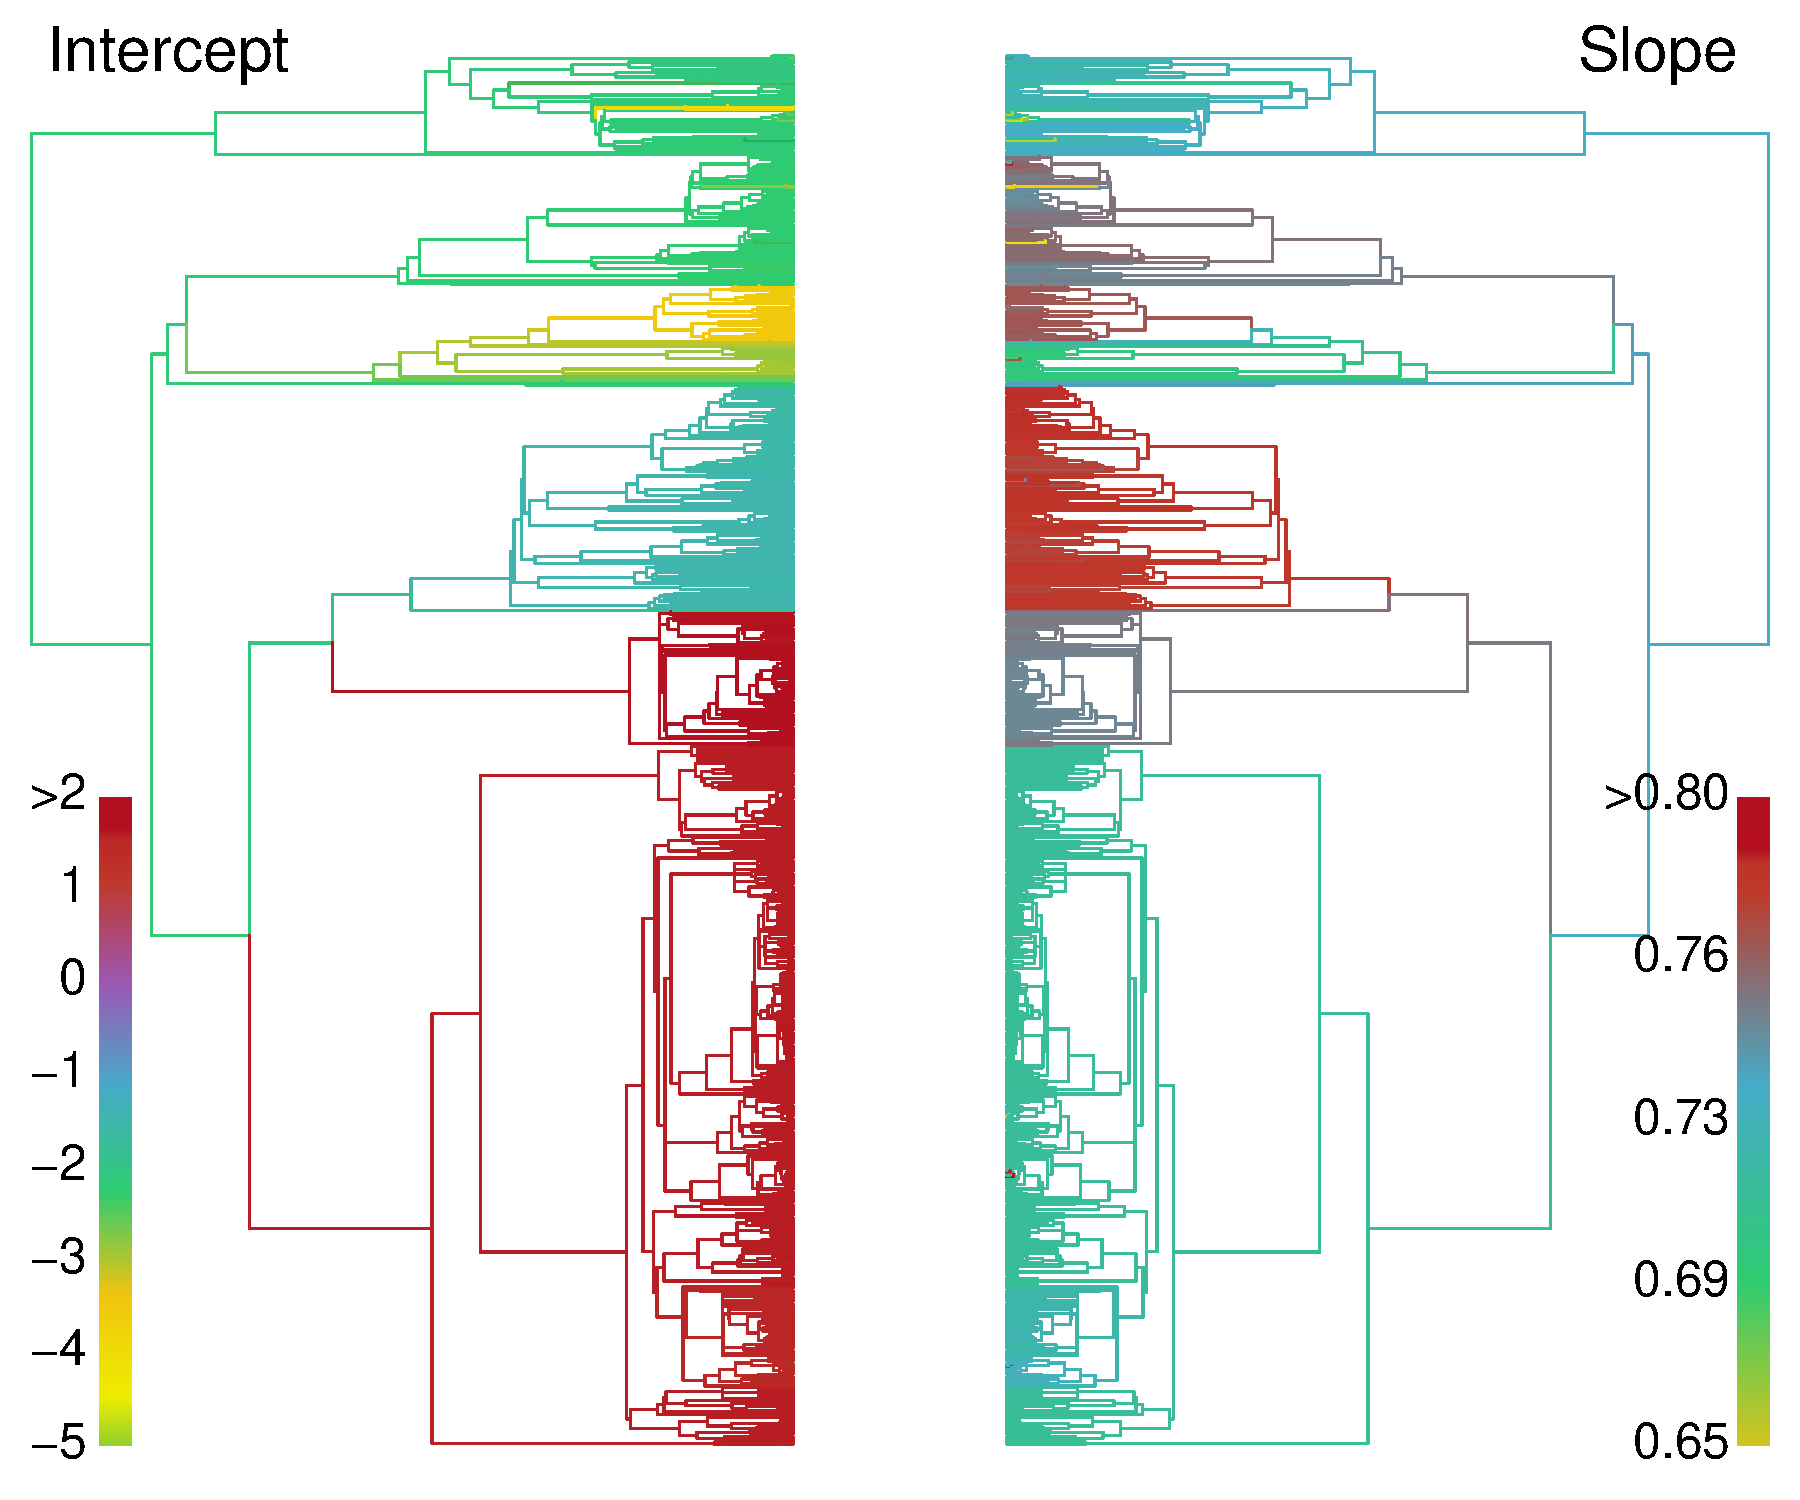
\includegraphics[scale=0.4]{figs/slopeint.pdf}
\caption{Slope intercept figure from reversible-jump run. (PUT PHYLOPIC IMAGES HERE ON WHITE-BACKGROUND FIGURE)}
\label{slopeint}
\end{figure}

\begin{figure}
\centering
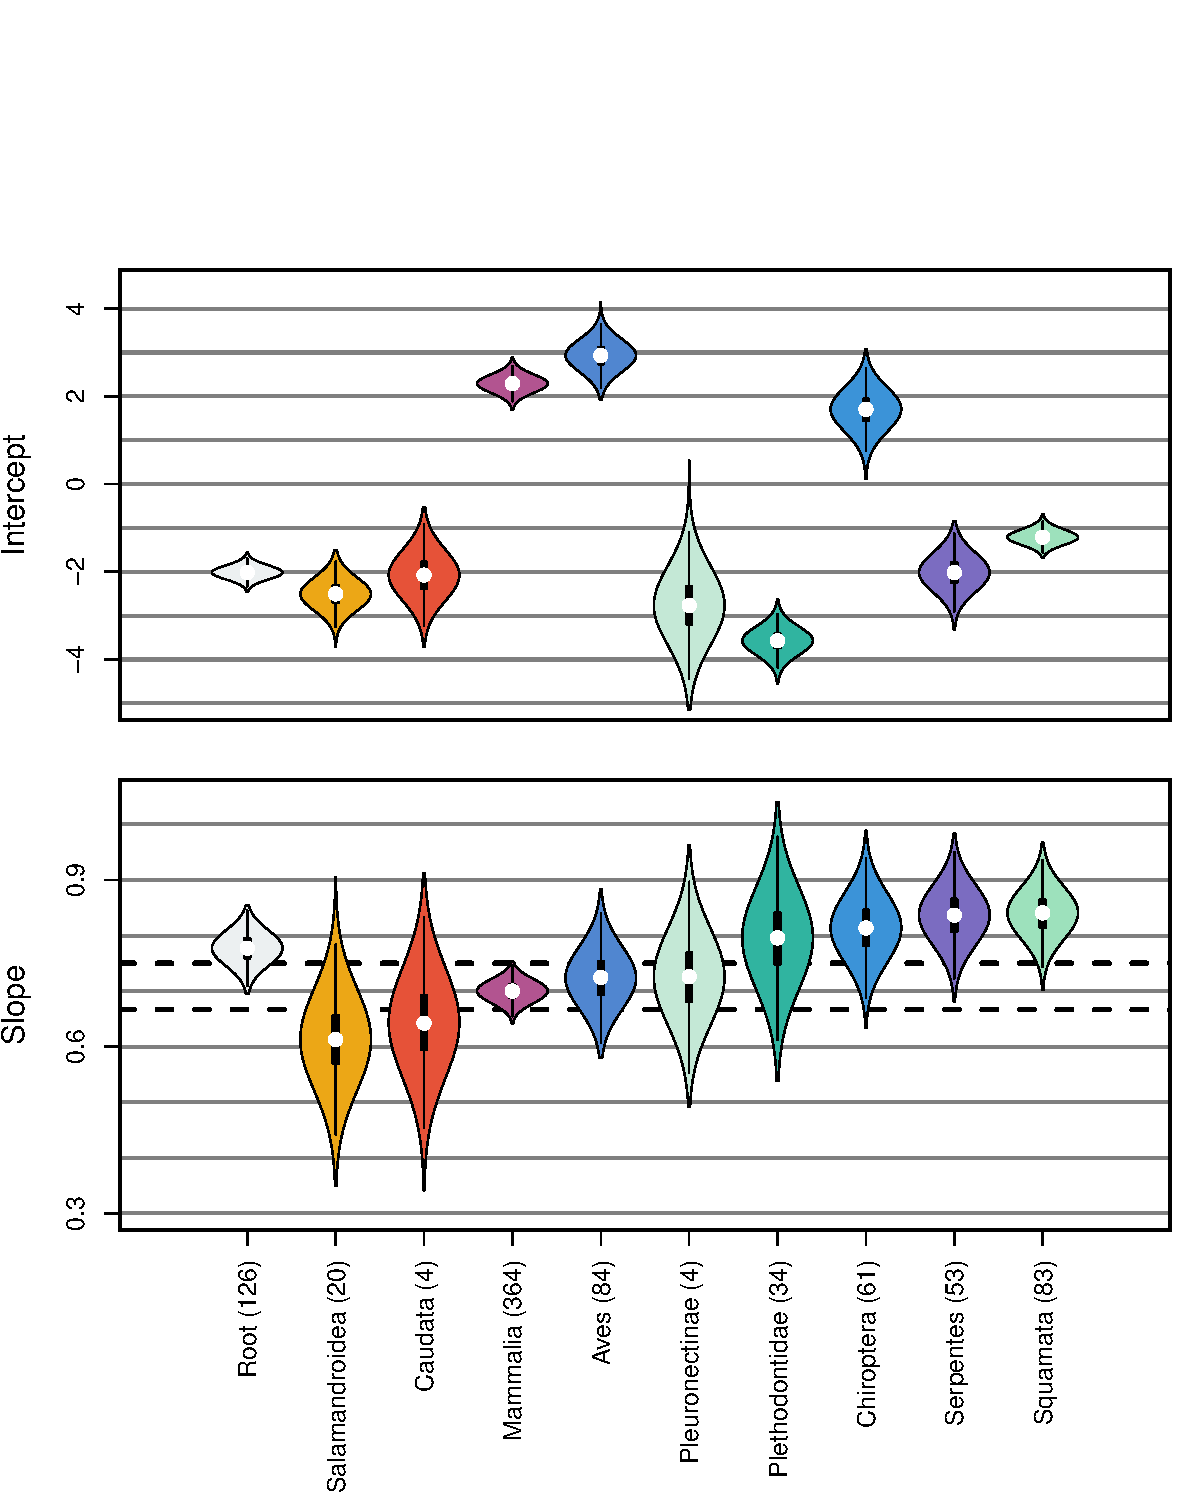
\includegraphics[scale=0.6]{figs/boxplots.pdf}
\caption{Parameter estimates for major identifies clades from the 4 fixed-shift chains with separate slopes and intercepts for each shift. Numbers in parentheses indicate the number of species in that group (that do not shift to another state). ADD PHYLOPICS.}
\label{boxplots}
\end{figure}

\begin{table}[p]
\begin{tabular}{l | r | r | r |}
Model &\ np.\ &\ Marginal lnL\ &\ Bayes Factor\ \\
\hline
$\theta + \beta_{endo} + \beta_{mass}$ & 5 & -702.20 & 249.1 \\
$\boldsymbol{\uptheta} + \beta_{endo}+\beta_{mass}$ & 33 & -633.60 & 111.9 \\
$\boldsymbol{\uptheta} + \beta_{endo}+\boldsymbol{\upbeta_{mass}}$ & 62 & -577.67 & 0 \\
$\boldsymbol{\uptheta} + \beta_{endo}+\beta_{mass} + \beta_{mass^2}$ & 34 & -635.98 &  116.6\\
$\boldsymbol{\uptheta} + \beta_{endo}+\boldsymbol{\upbeta_{mass}} + \beta_{mass^2}$ & 63 & -582.67 & 10.0 \\
$\boldsymbol{\uptheta} + \beta_{endo}+\beta_{mass} + \beta_{GS}$ & 35 & -633.04 & 110.7 \\
$\boldsymbol{\uptheta} + \beta_{endo}+\boldsymbol\upbeta_{mass} + \beta_{GS}$ & 65 & -582.77 & 10.2 \\
$\boldsymbol{\uptheta}^{-sal} + \beta_{endo}+\boldsymbol\upbeta_{mass}^{-sal} + \beta_{GS}$ & 58 & -589.13 & 22.9 \\
$\boldsymbol{\uptheta}^{-pleth} + \beta_{endo}+\boldsymbol\upbeta_{mass}^{-pleth} + \beta_{GS}$ & 63 &-584.42 & 13.5 \\
$\boldsymbol{\uptheta}^{-sal} + \beta_{endo}+\boldsymbol\upbeta_{mass}^{-sal} + \beta_{GS} + \beta_{GS \ \rm{X} \ \it{mass}}$ & 59 &-588.85  & 22.4 \\
$\boldsymbol{\uptheta}^{-pleth} + \beta_{endo}+\boldsymbol\upbeta_{mass}^{-pleth} + \beta_{GS} + \beta_{GS \ \rm{X} \ \it{mass}}$ & 64 & -592.60  & 29.9 \\

\end{tabular}
\caption{Model comparison}
\label{bf}
\end{table}

\renewcommand\thefigure{S.\arabic{figure}}
\renewcommand\thetable{S.\arabic{table}}


\begin{figure}
\centering
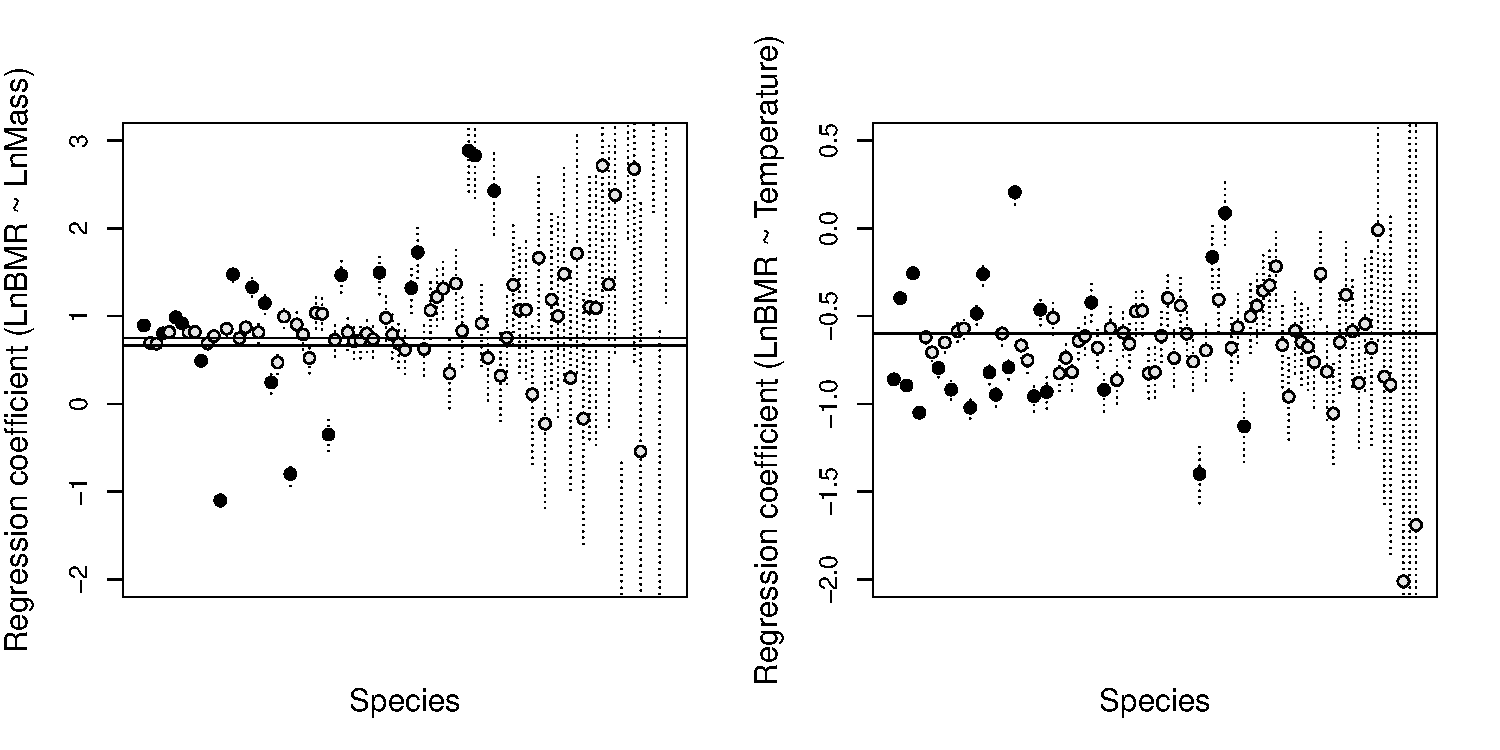
\includegraphics[scale=0.4]{figs/WithinSpeciesCoefficients.pdf}
\caption{Within-species scaling coefficients with mass (left) and temperature (right) estimated for species in the White dataset for which more than 3 measurements are available. }
\label{withincoef}
\end{figure}


%

\end{document}
